%% This is file `elsarticle-template-1-num.tex',
%%
%% Copyright 2009 Elsevier Ltd
%%
%% This file is part of the 'Elsarticle Bundle'.
%% ---------------------------------------------
%%
%% Ciência da Computação - UFRPE-UAG, Brasil.
%%
%% Antônio Adelino da Silva Neto, 2019.
%% Armstrong Lohãns de Melo Gomes Quintino, 2019.
%%
%% ---------------------------------------------

\documentclass[preprint,12pt,times]{elsarticle}

%% Use the graphicx package for more complicated commands
\usepackage{graphicx}

%% The amssymb package provides various useful mathematical symbols
\usepackage{amssymb}

%% The lineno packages adds line numbers. Start line numbering with
%% \begin{linenumbers}, end it with \end{linenumbers}. Or switch it on
%% for the whole article with \linenumbers after \end{frontmatter}.
\usepackage{lineno}

%% Usado para detectar PT-BR
\usepackage[brazilian]{babel}

%% Usado para detectar PT-BR
\usepackage[utf8]{inputenc}

%% Usado para detectar PT-BR
\usepackage[T1]{fontenc}

\usepackage{url}


\begin{document}

	\begin{frontmatter}

		%% Title, authors and addresses

		%% use the tnoteref command within \title for footnotes;
		%% use the tnotetext command for the associated footnote;
		%% use the fnref command within \author or \address for footnotes;
		%% use the fntext command for the associated footnote;
		%% use the corref command within \author for corresponding author footnotes;
		%% use the cortext command for the associated footnote;
		%% use the ead command for the email address,
		%% and the form \ead[url] for the home page:
		%%
		%% \title{Title\tnoteref{label1}}
		%% \tnotetext[label1]{}
		%% \author{Name\corref{cor1}\fnref{label2}}
		%% \ead{email address}
		%% \ead[url]{home page}
		%% \fntext[label2]{}
		%% \cortext[cor1]{}
		%% \address{Address\fnref{label3}}
		%% \fntext[label3]{}

		\title{Análise de algoritmos de reconhecimento de padrões}
				
		%% use optional labels to link authors explicitly to addresses:
		\author[a]{Antônio Adelino da S. Neto}
		\address[a]{antonio.asn03@gmail.com}
		
		\author[b]{Armstrong Lohãns de M. G. Quintino}
		\address[b]{lohansdemelo1108@gmail.com}
		
		\address{Garanhuns, Brasil}

		\begin{abstract}
			%% Text of abstract
			O objetivo principal desse trabalho foi a elaboração e o estudo de dois algoritmos para sistemas de aprendizado de máquina, os quais trabalhariam na classificação de textos em linguagem natural. Tais programas foram o algoritmo da Árvore de Decisão e o algoritmo de Naive Bayes. Inicialmente são mostrados os conceitos básicos sobre cada algoritmo de decisão acima citado. Depois haverá uma apresentação das técnicas usadas para a análise e as devidas conclusões.
		\end{abstract}

		\begin{keyword}
			Reconhecimento de Padrões \sep Árvore de Decisão \sep Naive Bayes
		\end{keyword}

	\end{frontmatter}

	%% Start line numbering here if you want
	\linenumbers

	%% Texto principal
	\section{Introdução}
	\label{Introdução}
	Os seres humanos e alguns outros animais possuem, entre outras habilidades, a aptidão no reconhecimento de padrões. O ser humano, especificamente, possui essa capacidade muito bem desenvolvida e tem uma enorme facilidade no reconhecimento formas, dando a elas significado e valor. Dentre elas pode-se citar a fisionomia de outros seres humanos, formas animais e vegetais, características pessoais e afins.

	Essa habilidade sempre foi muito importante, pois foi por meio dela que a espécie humana conseguiu desenvolver-se com mais facilidade ao longo do tempo, uma vez que ela permite a assimilação e inferência de características em formas aparentemente semelhantes. Partindo dessa premissa, é possível notar a relevância dessa aptidão em reconhecimento para o ser humano, em especial o reconhecimento de padrões, visto que é por meio dela que consegue-se inferir em formas desconhecidas julgamentos prévios a partir de conhecimentos anteriores.

	Com isso, afirma-se então que toda e qualquer forma de reconhecimento de padrões, por indivíduos, dá-se a partir de uma experiência passada. Dessa maneira é possível perceber que a destreza, ou não, no reconhecimento de padrões está diretamente vinculada aos estímulos que cada indivíduo foi submetido ao longo de sua vida \cite{Prado:2008}.

	Partindo dessas afirmativas, o presente artigo expõe um estudo que busca a análise comparativa de dois algoritmos. O algoritmo da Árvore de Decisão e o algoritmo de Naive Bayes, ambos voltados a classificação de dados baseando-se nos princípios de aprendizagem de máquina. 
	
	A análise desses algoritmos dá-se por meio da classificação de textos em linguagem natural, onde os classificadores recebem os textos e inferem a eles o sentido do que está escrito de acordo com classes anteriormente estabelecidas.
	

	\section{Referencial Teórico}
	\label{Referencial Teórico}

	\subsection{Algoritmo da Árvore de Decisão}

	As  Árvores de Decisão são técnicas muito populares de aprendizado de máquina, são aplicadas às tarefas de classificação e regressão. Esta técnica é caracterizada pelo seu modelo resultante, o qual é codificado como uma estrutura em árvore \cite{Nuti:2019}.

	As árvores de decisão são algoritmos que buscam a classificação dos dados a partir da estruturação em árvore. O algoritmo divide um conjunto de dados em subconjuntos menores. Sabendo que o código estrutura-se em árvore, cada nó folha representa uma decisão.

	Para chegar em uma decisão, o algoritmo comporta-se da seguinte maneira, com base nos valores dos recursos das instâncias, as árvores de decisão classificam os dados. Cada nó representa um recurso em uma instância da árvore de decisão que deve ser classificada, e cada ramo representa um valor \cite{Pandya:2015}.

	Sabendo disso, percebe-se que cada dado, para ser classificado, passa por um conjunto finito de nós, tal conjunto é definido como as regras de classificação, pois a partir desse conjunto é possível saber o passo a passo do algoritmo, mostrando assim todas as regras que levaram a classificação daquela única instância. A principal vantagem do uso das árvores de decisão está justamente na capacidade do retorno dos passos para a decisão e não unicamente no resultado da classificação.

	\subsection{Algoritmo de Naive Bayes}

	Além das árvores de decisão, pode-se também fazer uso de outros tipos de classificadores, entre eles destaca-se o Naive Bayes, o qual possui uma análise dos dados a partir de conceitos probabilísticos, diferenciando-se das árvores de decisão.
	
	O algoritmo de Naive Bayes é um classificador probabilísticos simples (baseado no Teorema de Bayes), tem como base em uma suposição comum de que todos os recursos são independentes um do outro \cite{xu:2018}. A partir disso, ele desconsidera completamente a correlação entre todas as variáveis, tratando cada variável de forma independente, esse algoritmo  é frequentemente aplicado em processamento de linguagem natural.
	
	Uma das principais vantagens do classificador Naive Bayes é que ele requer apenas uma pequena quantidade de dados iniciais de treinamento para poder estimar as médias e variações das variáveis necessárias para classificação \cite{vijayarani:2015}.
	
	\section{Ferramentas usadas}
	\label{Ferramentas usadas}
	
	\subsection{Linguagem Python}
	Antes de iniciar a implementação optamos por usar a linguagem de programação Python. Essa linguagem, além de ser uma das mais populares do mundo, é vastamente usada na produção de softwares e algoritmos voltados aos conceitos de aprendizagem de máquina, tanto no meio acadêmico quanto na indústria. 
	
	Pode-se afirmar também que a linguagem de programação Python é uma linguagem de fácil manipulação e de grande eficiência produtiva o que facilita todo o processo de codificação.
	
	\subsection{Módulo Sickit-Learn}
	Partindo dessa escolha inicial, foi possível utilizar o módulo Sickit-Learn para Python. Tal módulo integra em si uma grande quantidade de algoritmos de aprendizagem de máquina que são voltados para problemas supervisionados e não supervisionados \cite{scikit-learn}. 
	
	Além disso, essa biblioteca Python tem como característica a simplificação do uso de algoritmos de aprendizagem de máquina buscando a sua popularização. Essa difusão dá-se por meio da grande facilidade de uso, do bom desempenho e da sua documentação detalhada. Esse módulo ainda procura incentivar o seu uso, por meio de dependências mínimas e licença simplificada, em ambientes acadêmicos e comerciais de todo o mundo \cite{scikit-learn}.
	
	Diante dessas características encontradas na linguagem de programação Python e na biblioteca Sickit-Learn a implementação dos algoritmos, que servem de experimento para o presente artigo, tornou-se mais rápida e mais objetiva.
	
	\subsection{Wisdom Quotes (Base de dados)}
	Para a criação da base de dados inicial dos classificadores foi necessário a utilização do site \url{http://wisdomquotes.com} a fim de escolher textos aleatórios que fossem divididos por classificadores. O Wisdom Quotes conta com uma grade variedade de citações separadas por temas, permitindo a relação intuitiva citação-tema, o que vem a facilitar a criação e manipulação da base de dados dos classificadores.
	
	\section{Algoritmos}
	\label{Algoritmos}
	
	\subsection{Criação da base de dados}
	
	Antes de iniciar a implementação dos algoritmos brutos de aprendizado de máquina (Árvore de Decisão e Naive Bayes) tivemos que coletar as citações do site Wisdom Quotes. Para isso implementamos um script simples em Python (Crawler) que teve como finalidade apenas a coleta das citações do endereço URL que passamos e separar em arquivos de texto. 
	
	Com o Crawler o processo de coleta de dados tornou-se muito mais rápido e eficaz.
	A coleta foi feita em três páginas do mesmo site, cada página continha citações de uma única categoria, as três categorias foram escolhidas randomicamente e são elas:
	
	\begin{enumerate}
		\item Peace (do ingês, "Paz")
		\item Success (do ingês, "Sucesso")
		\item Silence (do ingês, "Silêncio")
	\end{enumerate}
	
	Com as citações salvas em arquivos de texto, tivemos que escolher aleatoriamente cento e cinquenta de cada classificador, a fim de deixar a base de dados uniforme, totalizando quatrocentos e cinquenta frases.
	
	A partir disso, armazenamos essas frases em dois vetores, o vetor de treino e o vetor de teste. Essas listas continham respectivamente sessenta por cento e quarenta por cento das citações, escolhidas aleatoriamente entre si. Essas porcentagens foram estabelecidas visando um melhor desempenho dos classificadores, uma vez que a quantidade de dados para treino é um pouco maior quando comparada a quantidade de dados para testes.
	
	\subsection{Árvore de Decisão}
	
	Com a base de dados inicial pronta, implementamos a arvore de decisão. Para usar a função de criação de uma árvore de decisão no Sickit-Learn é necessário inicialmente vetorizar as frases de teste, a função (também do Sickit-Learn) \textit{.fit\_transform()} do \textit{CountVextorizer()} vetoriza as frases em forma de matriz, além de contar a repetição de cada palavra na frase, trecho ilustrado na Figura 1. 
	
	\begin{figure}[h]
		\centering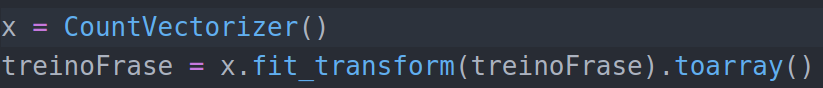
\includegraphics[width=0.7\linewidth]{Imagens/vetorizandoTeste.png}
		\caption{Vetorizando frases de teste.}
	\end{figure}
	
	 Com as frases devidamente vetorizadas, criamos a árvore de decisão a partir da função \textit{tree.DecisionTreeClassifier()} e a treinamos com o comando \textit{.fit(parm1, parm2)}, como mostrado na Figura 2, passando como parâmetro as frases vetorizadas e a lista de classificações. Cada frase vetorizada está localizada na posição de índice correspondente ao seu classificador que está na lista de classificadores.
	 
	 \begin{figure}[h]
		 \centering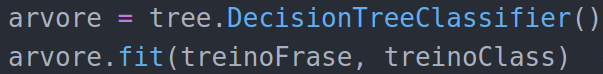
\includegraphics[width=0.7\linewidth]{Imagens/InstanciarArvore.png}
	 	\caption{Instanciando e treinando árvore de decisão.}
	 \end{figure}
	
	Após a criação da árvore, colocamos a base de testes para validar as classificações, a função \textit{.score(parm1, parm2)} retorna o percentual de acerto dos testes passados no segundo parâmetro, no primeiro parâmetro está o conjunto contendo todas as palavras conhecidas pela árvore (\textit{Bag of Words}), veja na Figura 3.
	
	\begin{figure}[h]
	\centering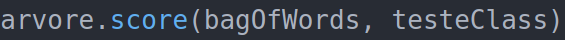
\includegraphics[width=0.7\linewidth]{Imagens/score.png}
	\caption{Função que retorna a porcentagem de acertos da estrutura.}
	\end{figure}

	Tendo a árvore de decisão montada também foi possível obter as regras de classificação citações passadas, para isso usamos a função, também do do Sickit-learn, \textit{.decision\_path()}, conforme mostra a Figura 4. 
	
	\begin{figure}[h]
	\centering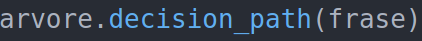
\includegraphics[width=0.7\linewidth]{Imagens/caminho.png}
	\caption{Função que retorna a as regras de decisão da árvore.}
	\end{figure}
	
	Com isso, terminamos a implementação do algoritmo da árvore de decisão e suas funcionalidades principais, dando destaque a possibilidade de listar o caminho de decisão de uma citação.
	
	\subsection{Naive Bayes}
	Para implementamos o classificador Naive Bayes no Sickit-Learn, foi necessário realizar o mesmo processo de vetorização das frases de teste, ilustrado na Figura 1. Tal processo teve como finalidade a vetorização das frases em forma de matriz enumerando a repetição de cada palavra da citação recebida, como já detalhado na subseção anterior.
		
	A partir disso, criamos a estrutura do Naive Bayes por meio da função \textit{GausianNB()} e a treinamos com o mesmo comando \textit{.fit(parm1, parm2)} usado no treino da árvore de decisão, como mostrado na Figura 5, passando como parâmetro as frases vetorizadas e a lista de classificações, semelhante ao que foi feito na árvore de decisão.
	
	\begin{figure}[h]
		\centering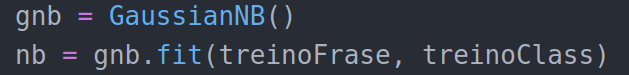
\includegraphics[width=0.7\linewidth]{Imagens/naive.png}
		\caption{Instanciando e treinando o algoritmo de Naive Bayes.}
	\end{figure}
	
	Depois de estruturar o Naive Bayes, colocamos a base de testes para validar as classificações, a função que faz isso é a mesma ilustrada na Figura 3 (\textit{.score(parm1, parm2)}), a qual tem como retorno o percentual de acerto dos testes passados.
	
	Com o algoritmo de Naive Bayes da biblioteca Sickit-Learn foi possível acessar as probabilidades de cada classe a partir do atributo \textit{gnb.class\_prior\_}, esse atributo é composto por uma lista com todas as probabilidades das classes, temos o acesso a essas classes a partir do atributo \textit{gnb.classes\_} que retorna uma lista com todas as classes, ambas as listas são organizadas de maneira que cada índice de uma delas esteja diretamente associado ao índice da lista seguinte, veja na Figura 6.
	
	\begin{figure}[h]
		\centering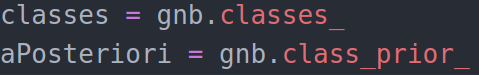
\includegraphics[width=0.7\linewidth]{Imagens/posteriori.png}
		\caption{Acesso aos atributos de  classe e probabilidade do Naive Bayes.}
	\end{figure}
	
	Dessa maneira terminamos a implementação do algoritmo de classificação Naive Bayes  e suas principais funções, dando relevância a possibilidade de listar as probabilidades a partir de cada classe.
	
	\subsection{Interação com o usuário}
	Após implementar os dois algoritmos de decisão acima descritos, elaboramos um pequeno algoritmo que permite ao usuário colocar em um campo de texto uma entrada e a partir dessa entrada o algoritmo retorna a sua classificação de acordo com os classificadores (\textit{Peace}, \textit{Success} e \textit{Silence}).
	
	A classificação é feita a partir de uma comparação de maior taxa de acertos na base de testes entre a árvore de decisão e o Naive Bayes, o que apresentar maior taxa de acerto terá a sua classificação mostrada ao usuário, Figura 7.

	\begin{figure}[h]
		\centering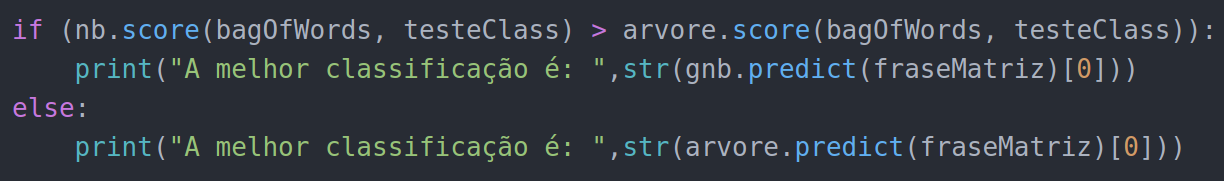
\includegraphics[width=0.7\linewidth]{Imagens/comp.png}
		\caption{Trecho de código para a tomada de decisão.}
	\end{figure}

	Além disso, o algoritmo retorna as regras de decisão da árvore e a probabilidade da classe, esse último a partir do Naive Bayes.
	
	Esse algoritmo ainda permite ser executado na própria base de testes retornando, com essa execução, a melhor classificação, as regras de decisão da árvore e a probabilidade da classe.
	
	\section{Análises e testes}
	\label{Análises e testess}
	
	\subsection{Árvore de Decisão}
	O primeiro teste realizado na árvore de decisão foi a validação dos dados de teste, os quais representavam quarenta por cento de toda a base de dados, como foi detalhado anteriormente. Para capturar as taxas de acerto usamos a função \textit{.score(parm1, parm2)}, também já descrita. 
	
	Os resultados obtidos a partir desse teste na árvore de decisão oscilaram por volta de quarenta por cento de taxa de acerto.
	
	Após essa primeira avaliação, testamos outra maneira de dividir e avaliar os dados, para isso entramos novamente no site \url{http://wisdomquotes.com} e coletamos o máximo de citações possíveis sobre os três classificadores escolhidos (\textit{Peace}, \textit{Success} e \textit{Silence}) e separamos em arquivos, usando o sript Crawler.
	
	Com esses novos dados fizemos uma validação cruzada usando uma função da biblioteca Sickit-Learn, a função \textit{cross\_val\_score(parm1, parm2, parm3, parm4)}), o qual recebe no primeiro parâmetro a estrutura do classificador, no segundo parâmetro recebe a base de dados, no terceiro parâmetro recebe os classificadores e no quarto parâmetro recebe a quantidade de subconjuntos que serão divididos os dados para treino e teste, veja na Figura 8. 
	
	\begin{figure}[h]
		\centering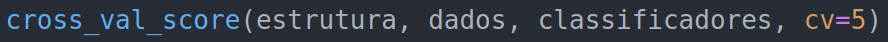
\includegraphics[width=0.7\linewidth]{Imagens/cruzada.png}
		\caption{Função de validação cruzada.}
	\end{figure}

	Para validarmos o classificador da árvore de decisão, adotamos o valor de cinco subconjuntos para fazer o teste. Com a validação cruzada dos cinco subconjuntos de dados a árvore de decisão trouxe uma média aproximada de sessenta por cento de acerto, um acréscimo de vinte por cento quando comparado ao primeiro teste.
	
	Testamos também mudança nas quantidades de subconjuntos para a análise, a partir de três subconjuntos a taxa média de acerto continuava por volta de sessenta por cento, entretanto notamos que quanto maior a quantidade de subconjuntos maior era a taxa de acerto, porém essa variação positiva foi extremamente pequena, para duzentos subconjuntos a porcentagem média foi de cerca de sesseta e quatro por cento, enquando com três subconjuntos essa média foi de cerca de sessenta e um por cento.
	
	\subsection{Naive Bayes}
	Semelhante ao que foi realizado na árvore de decisão, a validação dos dados de teste, os quais também representavam quarenta por cento de toda a base de dados, usamos a função \textit{.score(parm1, parm2)}, também já descrita e ilustrada na Figura 3. Essa função retorna a taxa de acerto do algoritmo quando ele é executado na base de testes. 
	
	Os resultados obtidos por meio desse teste no classificador Naive Bayes oscilaram em torno de trinta e cinco por cento.
	
	Depois dessa avaliação inicial e tendo novos dados coletados do site \url{http://wisdomquotes.com} separados pelos classificadores \textit{Peace}, \textit{Success} e \textit{Silence} fizemos uma validação cruzada, assim como feito na árvore de decisão, usando uma função \textit{cross\_val\_score(parm1, parm2, parm3, parm4)}), a qual já foi descrita e detalhada na subseção anterior (Figura 8).
	
	Adotamos o valor inicial de cinco subconjuntos para fazer o teste, baseando-se no experimento anterior da árvore de decisão. Com a validação cruzada dos cinco subconjuntos de dados o classificador Naive Bayes trouxe uma média de aproximadamente  quarenta e tês por cento de acerto, um acréscimo de quase dez por cento quando comparado ao primeiro teste.
	
	Entretanto realizamos também mudança nas quantidades de subconjuntos para a análise, e notamos que não houveram grandes diferenças quando modificamos a quantidade de subconjuntos no algoritmo de Naive Bayes, uma vez que os valores de acerto ficaram em torno de quarenta e cinco por cento.
	
	\section{Discussão dos resultados}
	\label{Discussão dos resultados}
	
	Com os resultados que foram obtidos pode-se inferir que os algoritmos de Naive Bayes e a Árvore de Decisão, apesar de eficientes, são muito dependentes da organização da base de dados.
	
	Com uma organização simples o desempenho dos dois algoritmos mostrou-se mais impreciso, a Árvore de Decisão com uma taxa de acerto por volta de quarenta por cento e o classificador Naive Bayes com uma taxa de acerto ainda menor, cerca de trinta e cinco por cento.
	
	Entretanto ao aplicarmos a validação cruzada, ambas as taxas tiveram um aumento significativo em suas referidas performances. A árvore de decisão teve um aumento de cerca de vinte por cento, enquanto o Naive Bayes teve um crescimento de dez por cento em sua taxa de acerto.
	
	Quanto ao tamanho da divisão dos subconjuntos da validação cruzada mostrou-se pouco relevante, o aumento ou diminuição da taxa de acerto ficaram em volta de dois por cento para mais ou para menos. 
	
	\section{Conclusão}
	\label{Conclusão}
	O presente artigo fez uma análise de dois algoritmos de classificação de dados em aprendizagem de máquina, o algoritmo da Árvore de Decisão e o algoritmo de Naive Bayes. Ambos mostraram-se capazes de inferir classificações a dados a partir de uma base de treino. 
	
	Entretanto os testes e análises feitos revelaram uma intima relação entre o poder de classificação e a maneira de estruturação e uso dessa base de dados. De forma que quanto mais tratados fossem os dados de treino e o seu uso, mais eficiente seria o classificador.
	
	Outro ponto importante de se destacar foi o melhor desempenho do algoritmo da árvore de decisão na classificação de linguagem natural, chegando a ter uma disparidade de dez por cento na taxa de acerto da classificação, se comparado ao algoritmo de Naive Bayes.
	
	As dificuldades encontradas no estudo foram decorrentes da adaptação dos dados em texto para que eles fossem aceitos pelas funções e métodos da biblioteca Sickit-Learn.
	
	Além disso, não conseguimos comparar as classificações com noventa e cinco por cento de confiança nem inferir testes de hipóteses aos classificadores.
	
	Por fim, o presente estudo conclui que cada um dos algoritmos tem sua respectiva peculiaridade, na árvore de decisão destacamos a possibilidade de obter as regras de decisão ao fim da classificação, enquanto no Naive Bayes destacamos a oportunidade de conseguir a probabilidade de cada classificação. Assim mostrando que os algoritmos de aprendisagem de máquina são versáteis e plurais, permitindo ao programador desfrutar de características específicas de um ou de outro para moldar a solução do seu problema.
		
	%% References with bibTeX database:
	\bibliographystyle{model1-num-names}
	\bibliography{bibliografia}

\end{document}
